\documentclass[12pt,a4paper]{article}
\usepackage[utf8]{inputenc}
\usepackage{amsmath}
\usepackage{amsfonts}
\usepackage{amssymb}
\usepackage{graphicx}

\usepackage{pgfplots}
\pgfplotsset{compat=1.16}
\usepackage{tikz}


\usepackage[left=2cm,right=2cm,top=2cm,bottom=2cm]{geometry}
\usepackage{fancyhdr}
\pagestyle{fancy}

\fancyhf{}
\lhead {Mr SABOUR}
\chead{Mouvement d'un projectile dans l'air}
\rhead {2ème Bac SM}
\lfoot{fiches de Mr SABOUR pour $2\textsuperscript{ème}$ bAC  SM }
\rfoot{\thepage}
\renewcommand{\footrulewidth}{0.05pt}

\begin{document}
\begin{minipage}{9cm}

HIBA muni de son fusil qui a la possibilité de lancer des balles de masse $m$ à partir d’un point $O$ origine du repère  $R(o,;\vec{i},\vec{j})$ 
avec une vitesse initiale $\vec{V_0}$ formant un angle $\alpha$ avec  l'horizontal, veut atteindre une cible  $C(X_C,Y_C)$. Prendre  $g= 10  m.s^{-2}$

\subsection*{partie I : la balle est considérée en chute libre }

\begin{enumerate}
\item Appliquer la $2\textsuperscript{ème}$ loi de Newton  et trouver l'équation de la trajectoire $y=f(x)$
\item Trouver l'expression de la flêche h (l'ordonnée du sommet de la trajectoire)et la portée D ( abscisse de point de rencontre avec l'axe $(OX)$ en fonction de $g,\alpha ,V_0$.

\end{enumerate}
\end{minipage}
\begin{minipage}{8cm}

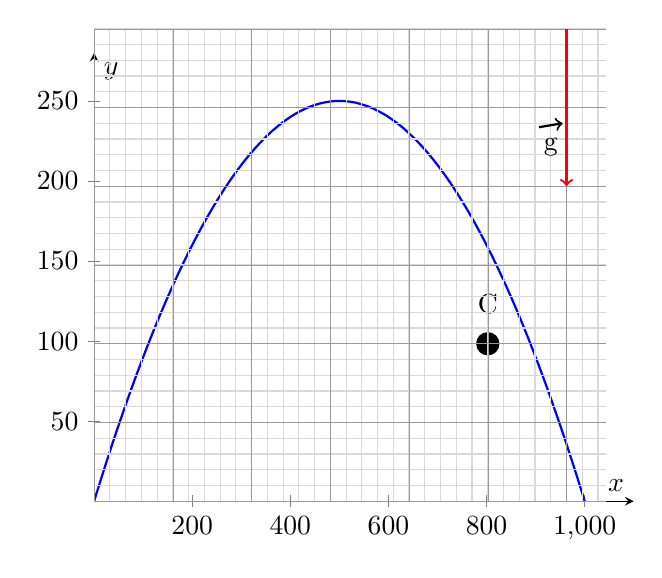
\begin{tikzpicture}
\begin{axis}[
    xlabel={$x$},
    ylabel={$y$},
    xmin=0,xmax=1100,
    ymin=0,ymax=280,
    axis lines=middle,
    domain= 0:1200,
    samples=100]
\addplot[blue,thick]{-0.001*x^2+x};
\end{axis}
\filldraw[black] (5,2) circle (4pt);
 \node at (5,2.5) {C};
 \draw[step=0.2cm,gray!30,thin](0,0)grid(6.5,6);
\draw[step=1cm,gray!80,very thin]( 0,0) grid (6.5,6);
  \draw[->,red,thick] (6,6) -- (6, 4);
  \node at (5.8,4.5) {g};
   \draw[->,black,thick](5.65,4.75) -- (5.95,4.8);
\end{tikzpicture}
\end{minipage}
\begin{enumerate}
 \item[3.] la courbe ci-contre représente les trajectoire du mobile. Montrer que $ V_0=100m.s^{-1}$ et  $\alpha = 45^\circ$. 
 \item[4.] On désire que le projectile passe par la cible $C(X_C,Y_C)$
 \begin{enumerate}
 \item Montrer qu'il existe une courbe appelée courbe de sûreté à l'extérieur de laquelle la cible est en sécurité par contre si elle est à l'intérieur, elle peut être atteinte de deux façons 
 \item Trouver la relation entre les deux façons si elle est au sol.
\item Avec une vitesse initiale $V_0=100m.s^{-1}$ quelles sont les angles du tir qui pour atteindre la cible si elle est situé au point $ C_0(0.8 km,100 m)$
 \end{enumerate}
 \subsection*{partie II : mouvement avec frottement fluide }
 en réalité les balles sont suffisamment dense qu'on peut négliger la poussée d'Archimède.mais leurs vitesse très grandes qui font que la force de frottement fluide ne peut être négligée; on la modélise par une force $\vec{f}=-k\vec{v}$
  \item[5.] en appliquant  la $2\textsuperscript{ème}$ loi de Newton, montrer que les équations différentielles vérifiés par $v_x$ et $v_y$ sont : 
\begin{equation*}
\left\{
\begin{aligned}
&\tau\frac{dv_x}{dt}+v_x=v_{lx}\\
& \tau\frac{dv_y}{dt}+v_y=v_{ly}
\end{aligned}
\right.
\end{equation*}
\item[6.] Donner alors les caractéristiques de $v_{limite}$
\item[7.] La solution de l'équation différentielle
 $\tau\frac{df}{dt}+f=f_l$ est $f(t)=(f(0)-f_l)e^{-\frac{t}{\tau}}+f_l$. 
donner les expressions de  $v_x(t)$ et $v_y(t)$ 
\item[8.]En déduire ,par intégration,les expressions de $x(t)$ et $y(t)$ 
\item[9.]Montrer que l'équation de la trajectoire est :$$y(x)=(\tan \alpha+\frac{mg}{kv_0 .cos\alpha})x + \frac{m^2g}{k^2}\ln (1-\frac{kx}{mv_0 .cos\alpha})$$

\end{enumerate}
 \end{document}
